%!TEX root = /Users/louis/Documents/PhD/Deliverables/ThesisOutline/thesis_outline.tex

\subsection{Revised Plan}
\label{subsec:plan}
A revised research plan is provided overleaf. I have found the plan in the progress report to be more effective than the plan in the qualifying dissertation. Defining clear goals, and decomposing large activities into smaller activities, increased my focus. I have continued to apply these techniques to produce the plan shown overleaf. A final plan for activities starting after January 2010 will be presented at the thesis audit.

\clearpage
\setlength\paperheight{297mm}
\setlength\paperwidth{420mm}
\setlength\pdfpageheight{\paperheight}
\setlength\pdfpagewidth{\paperwidth}

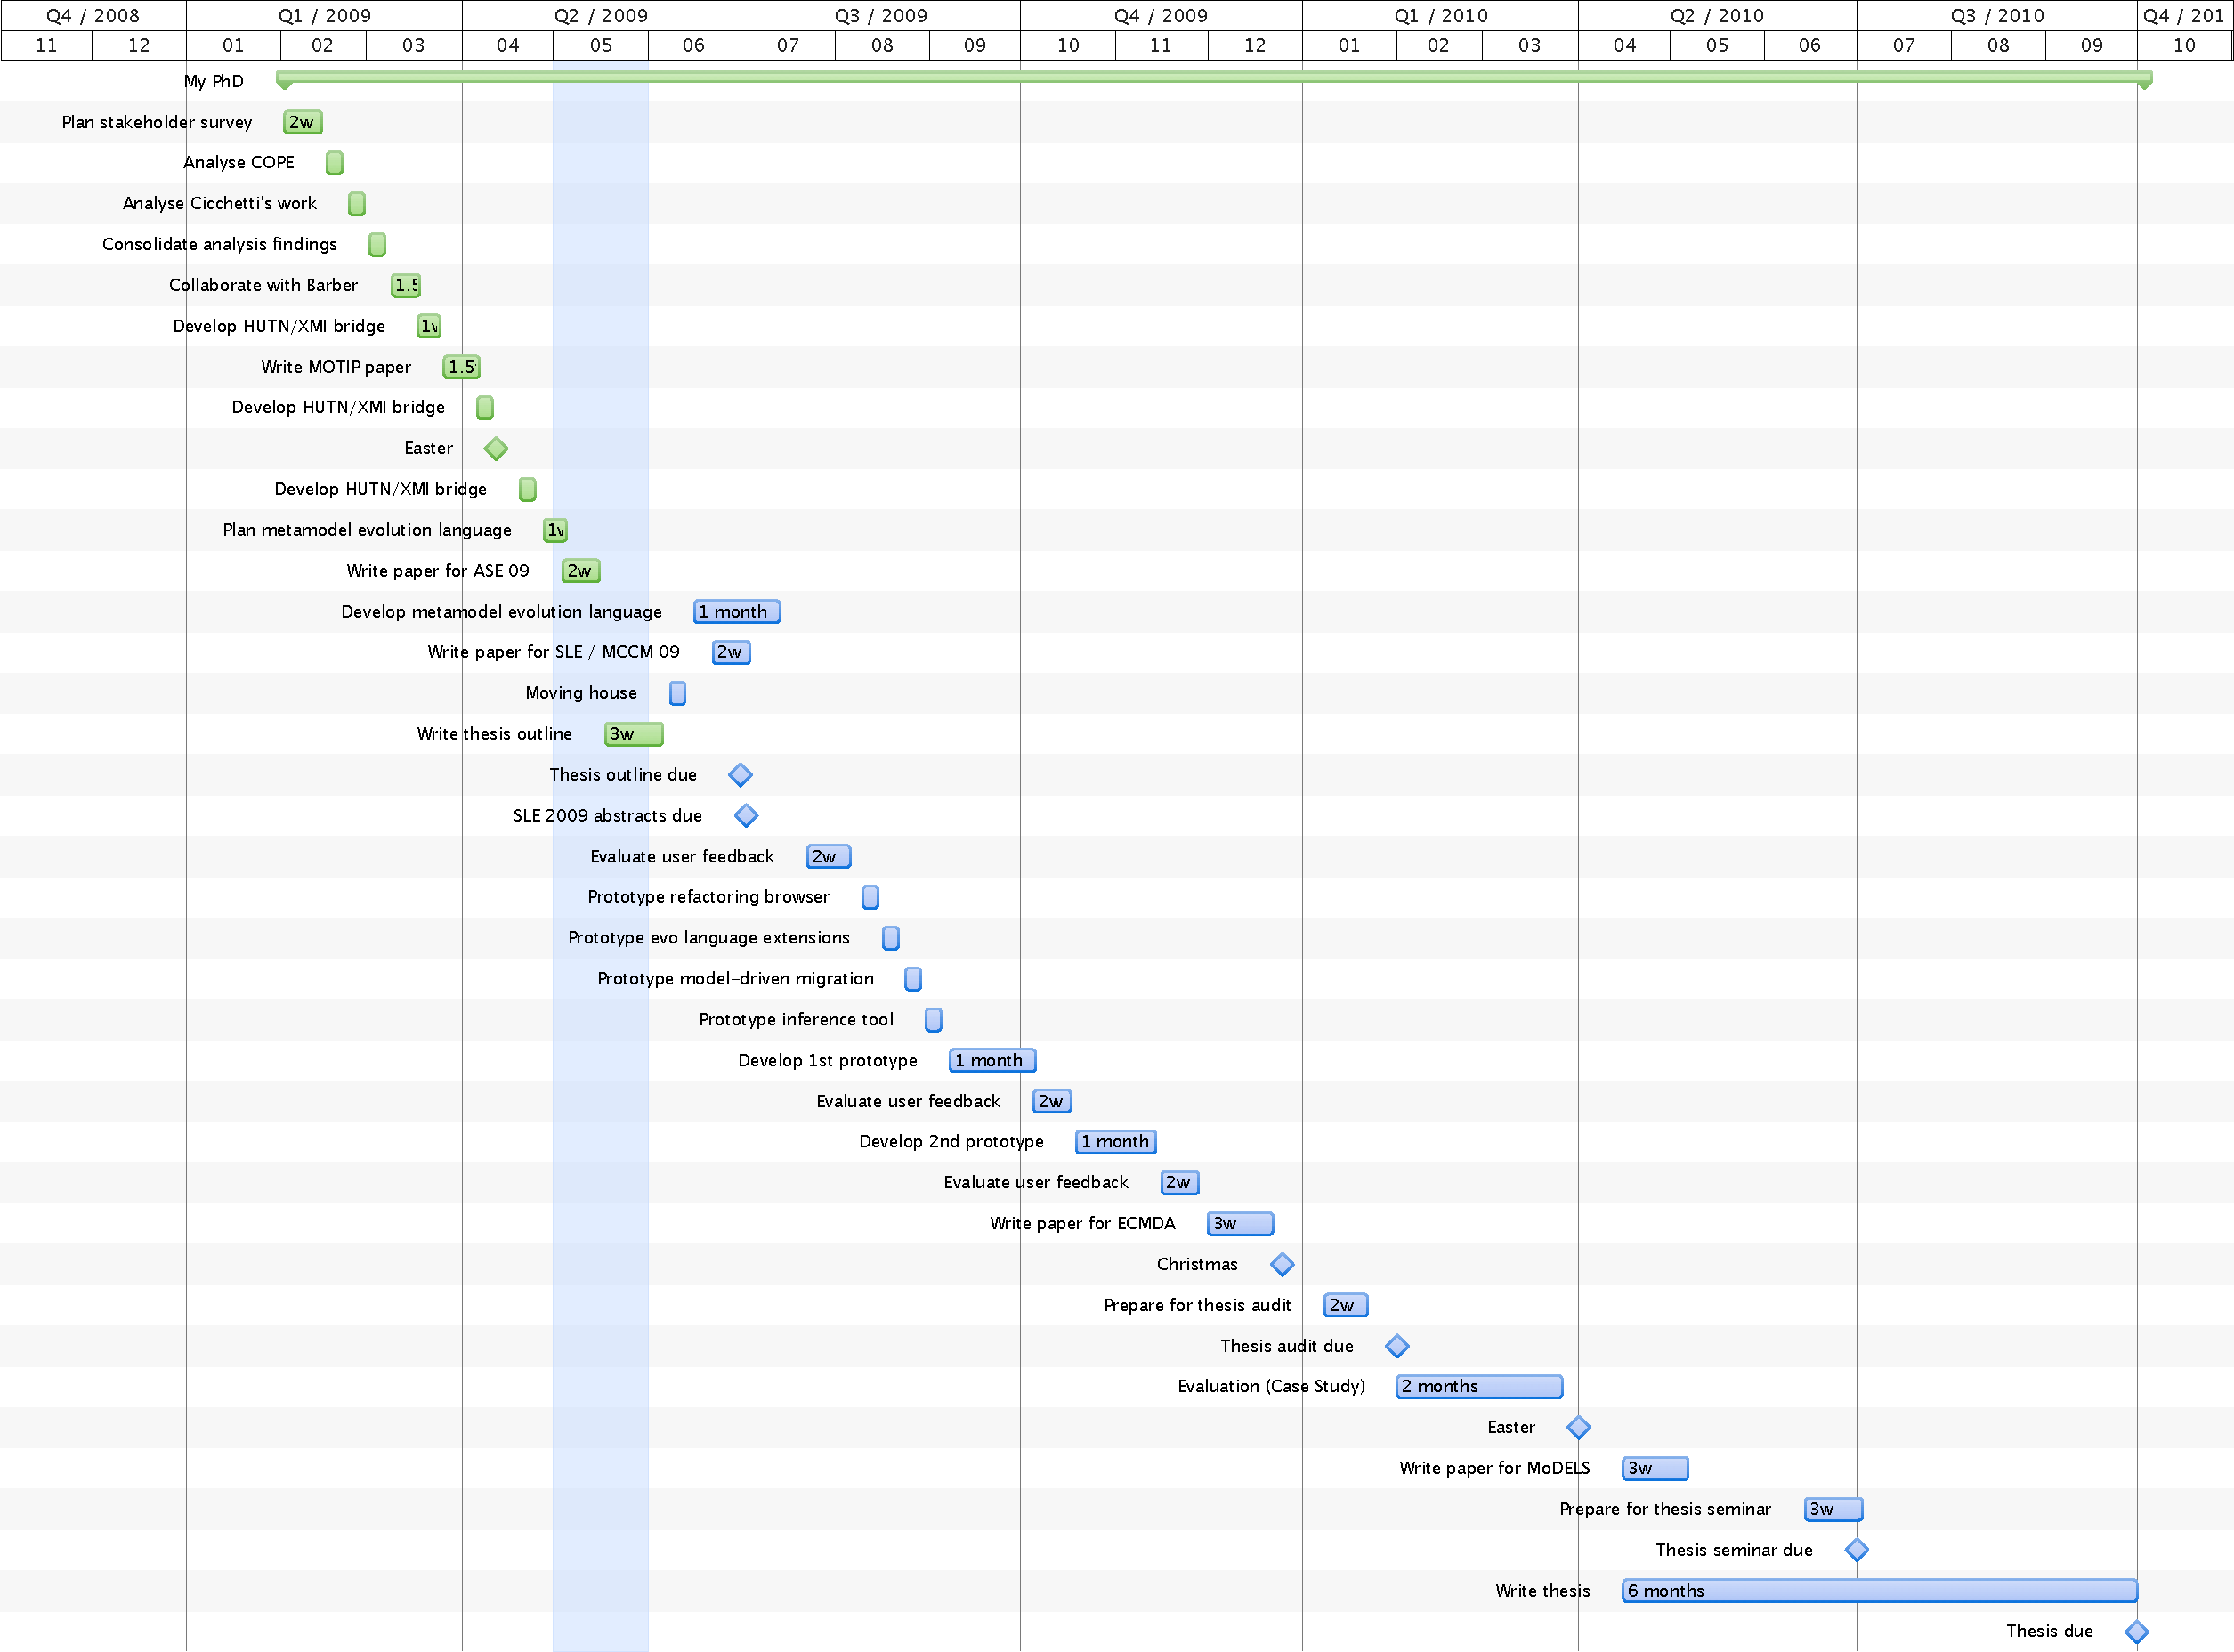
\includepdf[scale=1, pages={1}, addtolist={1,figure,{foo},fig:old_plan,2,figure,{foo},fig:revised_plan}]{Plan.pdf}

\setlength\paperheight{297mm}
\setlength\paperwidth{210mm}
\setlength\pdfpageheight{\paperheight}
\setlength\pdfpagewidth{\paperwidth}

\subsection{Goals} % (fold)
\label{sub:goals}
Over the next six months, our primary goal is to address the requirements we have defined for managing co-evolutionary changes in the context of model-driven engineering. Specifically, we will develop a language for describing and executing migration strategies, and other structures and processes that will automate some of the development activities that occur during model and metamodel co-evolution.

Our research will be evaluated using the Graphical Modelling Framework (GMF) \cite{gronback06gmf} as a case study. We will demonstrate that those problems occurring in GMF caused by co-evolutionary change can be managed using the structures and processes that we develop.

\paragraph{Develop model migration language}
In the progress report, we motivated the need for a dedicated language for specifying and executing model migration. By analysing existing examples of co-evolution, we have designed a minimal core syntax for the language. Over the next month, we will choose an implementation strategy (internal extension to a general purpose language, or new task-specific language for Epsilon) and a target platform (e.g. Ruby, Scala, Epsilon). We will then implement the model migration language and development tools. The work will produce publishable results, possibly in time for submission to the 2nd International Conference on Software Language Engineering (SLE), or to the 2nd International Workshop on Model Co-Evolution and Consistency Management (MCCM).

\subparagraph{Goals:} Choose an implementation strategy and target platform. Implement the language. Publish a paper at SLE / MCCM 09.


\paragraph{Evaluate user feedback}
The model migration language will be released as part of the Epsilon research incubation project. Potentially, users will provide feedback and suggest improvements. Clearly, it is difficult to predict the amount of user feedback we will receive. Regardless, we have planned some time for improving the language in response to user feedback.

\subparagraph{Goals:} Improve the model migration language based on user feedback.


\paragraph{Prototyping and further development}
In Section~\ref{subsubsec:further_solutions}, we identified several further solutions that could be implemented to address the requirements of structures and processes for managing co-evolutionary change in the context of MDE. We have planned time to rapidly prototype each of the solutions. Time has been planned for further development of two of the prototypes. The developed solutions and the prototypes will provide content for the proposed thesis. One or both of the developed prototypes will likely be publishable.

\subparagraph{Goals:} Prototype the solutions discussed in Section~\ref{subsubsec:further_solutions}, selecting two of them for further development. Develop the chosen two solutions. Publish a paper at ECMDA 2010.